\subsection{Generalizations of Dyck words: Motzkin, Schröder, and Łukasiewicz paths}
Motzkin, Schröder, and Łukasiewicz paths provide generalizations of Dyck words.  

In addition to representing balanced parentheses, Dyck paths can be thought of as paths on a cartesian plane.  Dyck paths are paths from $(0,0)$ to $(2n,0)$ that use $2n$ steps of either $(1,1)$ (northeast) or $(1,-1)$ (southeast) and never cross below the x axis. In the binary string representation of Dyck words, ones correspond to $(1,1)$ steps and zerores correspond to $(1,-1)$ steps.

Motzkin paths allow for (1,0) horizontal steps in addition to (1,1) and (1,-1) steps. Schröder paths are identical to Motzkin paths except they allow for $(2,0)$ horizontal steps instead of $(1,0)$.  Łukasiewicz paths allow (1,-1) steps, (1,0) steps and any (1,k) step where k is a positive integer.  All three languages retain the requirement that the path start at the origin, end on the x axis, and never step below the x axis. 

These paths can be encoded in a number of different ways.  In a \emph{-1-based encoding}, each $(1,i)$ step is encoded as i, and every prefix must have a nonnegative sum.  In a \emph{0-based encoding}, each $(1,i)$ step is encoded as $i+1$, and the sum of every prefix must be as large as its length. We primarily use the 0-based encoding. See Fig. \ref{paths}  for examples of these paths using the 0-based encoding.

We refer to Motzkin, Schröder, and Lukasiewicz paths ending at $(n,0)$ as paths of \emph{order n}.  This contrasts slightly with the classification of Dyck words of order n, which terminate at $(2n,0)$

In the context of fixed-content generation, Motzkin and Schröder paths are identical:  Both will have northeast steps encoded as twos, horizontal steps encoded as ones, and southeast steps encoded as zeroes.  However, their graphical representations Notably, Łukasiewicz are a generalization of Motzkin and Schröder paths, as any Motzkin or Schröder path is also a Lukasiewicz path.

\bigskip

\begin{figure}[]
	\centering
	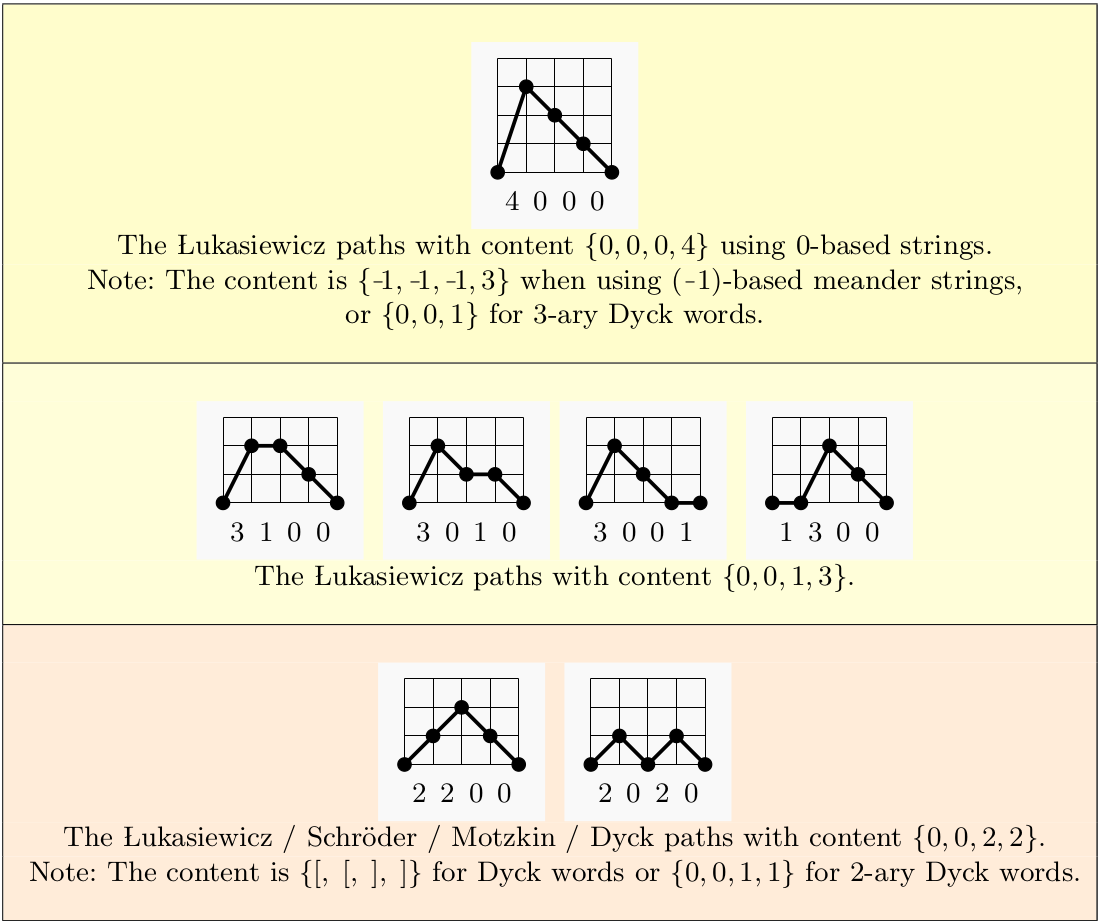
\includegraphics[width = .95 \textwidth]{paths.png}
	\caption{}
	\label{paths}
\end{figure}


The number of Dyck words with n zeroes and n ones are counted by the nth Catalan number.  Similarly, the number of Motzkin and Schröder paths of order n are counted by the nth Motzkin and big Schröder number respectively. The number of Lukasiewicz paths of order n are counted by the n
Motzkin, Schröder, and Lukasiewicz paths bear a number of interesting bijective correspondences with other combinatorial objects. Richard Stanely's \emph{Catalan Objects} outlines hundreds of interesting examples.  

Lukasiewicz paths  of order n bear a particularly nice correspondence to rooted ordered trees with $n+1$ nodes. See Fig. \ref{trees} for an illustration of this.

\begin{figure}[]
	\centering
	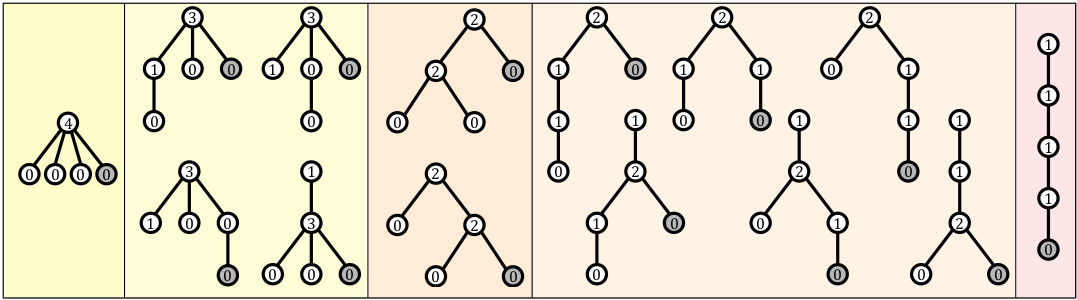
\includegraphics[width = .95 \textwidth]{trees.png}
	\caption{The $\mathcal{C}_4$=14 Lukasiewicz paths of order $n=4$ are in bijective correspondence with the 14 rooted ordered trees with $n+1=5$ nodes.  Given a tree, the corresponding word is obtained by recording the number of children of each node in preorder traversal; the zero from the rightmost leaf is omitted.  For example, the two trees in the middle section correspond to 2200 (top) and 2020 (bottom) respectively.}
	\label{trees}
\end{figure}

